\documentclass[11pt]{amsart}


%The package below let's us add todos to the document in a way that will stand out at a glance.  It will also list all of the current things to do, with their respective page numbers on the first page of the document.  You can add a todo like this:
%
%		Text text text \todo{change this text to something useful!}
%
%Among other things, you can edit the color of a todo:
%
%		\todo[color=\ltblue]{this todo will have a light blue background!}
%
%And you can include the todo as a line in the text, rather than in the margins:
%
%		\todo[inline]{this will appear in the middle of the page}

\usepackage[colorinlistoftodos, textsize=tiny]{todonotes}
\def\ltblue{blue!20!white}
\def\ltgreen{green!20!white}

\usepackage{amsmath,amssymb,amsthm, MnSymbol}
\usepackage{enumerate}
\usepackage{natbib}

\usepackage{tikz}
\usepackage{tikz-cd}
\usetikzlibrary{matrix, calc, arrows}
\usepackage{latexsym,amscd,epsfig,verbatim}
\usepackage[margin=1in,letterpaper,portrait]{geometry}

\newtheorem{thm}{Theorem}[section]
\newtheorem{lem}[thm]{Lemma}
\newtheorem{prop}[thm]{Proposition}
\newtheorem{cor}[thm]{Corollary}
\newtheorem{conj}[thm]{Conjecture}

%\usepackage[all]{xy}
\theoremstyle{definition}
\newtheorem{defn}[thm]{Definition}
\newtheorem{rem}[thm]{Remark}
\newcommand\fri{s_4^{-1}}
\newcommand\fr{s_4}
\newcommand\tri{s_3^{-1}}
\newcommand\tr{s_3}
\newcommand\twi{s_2^{-1}}
\newcommand\tw{s_2}
\newcommand\oni{s_1^{-1}}
\newcommand\on{s_1}

\makeatletter
\providecommand\@dotsep{5}
\def\listtodoname{List of Todos}
\def\listoftodos{\@starttoc{tdo}\listtodoname}
\makeatother


\begin{document}

%This adds the list of todos to the first page.
\listoftodos


\section{Diagrams of Finite Type}

In this section, we shall review the structure of diagrams of finite type, and how their cycles are effected by mutation. This section is simply a recap of \cite[Section 2]{BM13}.

\begin{defn}
A {\it chordless cycle} of an unoriented graph $G$ is a connected subgraph $H \subset G$ such that the number of vertices in $H$ is equal to the number of edges in $H,$ and the edges in $H$ form a single cycle.  
\end{defn}

\begin{prop}
Let $\Gamma$ be a diagram of finite type. Then, a chordless cycle in the unoriented graph of $\Gamma$ is cyclically oriented in $\Gamma$. Furthermore, the unoriented graph underlying the cycle must either be a cycle such that all edges have weight 1, a triangle with two edges of weight 2 and one of weight 1, or a square with two opposite edges of weight 2 and two opposite edges of weight 1, as pictured below.

\begin{tikzpicture}[baseline=-0.5ex]
 \matrix[matrix of math nodes,column sep={40pt,between origins},row
    sep={40pt,between origins},nodes={asymmetrical rectangle}] at (0,0)
  {
    & &|[name = ul]|\circ& |[name = ur]|\circ&\\
    %
    &|[name=lu]| \circ &&&|[name=ru]| \circ \\
     & |[name = ld]|\circ&&& |[name = rd]|\circ\\
    %
    &&|[name=dl]| \circ &|[name=dr]| \circ &\\
  };
\draw
  (ul) -- node[above] {1} (ur)
  ;
  \draw
  (ul) -- node[left]{1}(lu)
  ;
  \draw
  (dr) -- node[right]{1}(rd)
  ;
  \draw
  (lu) -- node[left]{1}(ld)
  ;
  \draw
  (ru) -- node[right]{1}(rd)
  ;
  \draw
  (ur) -- node[right]{1}(ru)
  ;
  \draw
  (dl) -- node[left]{1}(ld)
  ;
  \draw[dotted]
  (dl) -- (dr)
  ; 
 \matrix[matrix of math nodes,column sep={40pt,between origins},row
    sep={40pt,between origins},nodes={asymmetrical rectangle}] at (6,0)
  {
    & |[name = ul]|\circ& |[name = ur]|\circ\\
    %
    &|[name=dl]| \circ &|[name=dr]| \circ \\
  };
\draw
  (ul) -- node[above] {1} (ur)
  ;
  \draw
  (dl) -- node[left]{2}(ul)
  ;
  \draw
  (dr) -- node[below]{1}(dl)
  ;
  \draw
  (ur) -- node[right]{2} (dr)
  ; 
   \matrix[matrix of math nodes,column sep={25pt,between origins},row
    sep={40pt,between origins},nodes={asymmetrical rectangle}] at (10,0)
  {
    && |[name = u]|\circ& \\
    %
    &|[name=dl]| \circ & &|[name=dr]| \circ \\
  };
\draw
  (u) -- node[right] {2} (dr)
  ;
  \draw
  (dl) -- node[left]{2}(u)
  ;
  \draw
  (dr) -- node[below]{1}(dl)
  ;
  
   \end{tikzpicture}

\end{prop}
\begin{proof}
See \cite[Proposition 2.1]{BM13}.
\end{proof}

\begin{lem}
Let $\Gamma$ be a diagram of finite type with $\Gamma' = \mu_k(\Gamma)$ the mutation of $\Gamma$ at vertex $k.$ Below, we list induced subdiagrams in $\Gamma$ on the left and the resulting induced subdiagrams in $\Gamma'$ with chordless cycles $C'$ on the right, after mutation at $k.$ We draw the diagrams so that $C'$ always has a clockwise cycle. Furthermore, in case $(i),$ we assume $C'$ has at least three vertices, while in case $(j),$ we assume $C'$ has at least four vertices. Every chordless cycle in $\Gamma'$ is of one of these types.

\begin{enumerate}[(a)]
\item 	
	\begin{tikzpicture}[baseline=-0.5ex]
	 \matrix[matrix of math nodes,column sep={25pt,between origins},row
    sep={40pt,between origins},nodes={asymmetrical rectangle}] at (0,0)
  {
    && |[name = u]|\bullet& \\
    %
    &|[name=dl]| \circ & &|[name=dr]| \circ \\
  };
\draw[->]
  (dr) to node[right] {1} (u)
  ;
  \draw[->]
  (u) to node[left]{1}(dl)
  ;
  \node [yshift = .4 cm] at (u){k=2};
    \node [yshift = -.4 cm,xshift = .4 cm] at (dr){3};
    \node [yshift = -.4 cm,xshift = -.4 cm] at (dl){1};
    \matrix[matrix of math nodes,column sep={25pt,between origins},row
    sep={40pt,between origins},nodes={asymmetrical rectangle}] at (6,0)
  {
    && |[name = u]|\bullet& \\
    %
    &|[name=dl]| \circ & &|[name=dr]| \circ \\
  };
\draw[->]
  (u) to node[right] {1} (dr)
  ;
  \draw[->]
  (dl) to node[left]{1}(u)
  ;
  \draw[->]
  (dr) to node[below]{1}(dl)
  ;
  \node [yshift = .4 cm] at (u){k=2};
    \node [yshift = -.4 cm,xshift = .4 cm] at (dr){3};
    \node [yshift = -.4 cm,xshift = -.4 cm] at (dl){1};
   \end{tikzpicture}
   \item 	
	\begin{tikzpicture}[baseline=-0.5ex]
	 \matrix[matrix of math nodes,column sep={25pt,between origins},row
    sep={40pt,between origins},nodes={asymmetrical rectangle}] at (0,0)
  {
    && |[name = u]|\bullet& \\
    %
    &|[name=dl]| \circ & &|[name=dr]| \circ \\
  };
\draw[->]
  (dr) to node[right] {1} (u)
  ;
  \draw[->]
  (u) to node[left]{2}(dl)
  ;
  \node [yshift = .4 cm] at (u){k=2};
    \node [yshift = -.4 cm,xshift = .4 cm] at (dr){3};
    \node [yshift = -.4 cm,xshift = -.4 cm] at (dl){1};
    \matrix[matrix of math nodes,column sep={25pt,between origins},row
    sep={40pt,between origins},nodes={asymmetrical rectangle}] at (6,0)
  {
    && |[name = u]|\bullet& \\
    %
    &|[name=dl]| \circ & &|[name=dr]| \circ \\
  };
\draw[->]
  (u) to node[right] {1} (dr)
  ;
  \draw[->]
  (dl) to node[left]{2}(u)
  ;
  \draw[->]
  (dr) to node[below]{2}(dl)
  ;
  \node [yshift = .4 cm] at (u){k=2};
    \node [yshift = -.4 cm,xshift = .4 cm] at (dr){3};
    \node [yshift = -.4 cm,xshift = -.4 cm] at (dl){1};
   \end{tikzpicture}
   \item 	
	\begin{tikzpicture}[baseline=-0.5ex]
	 \matrix[matrix of math nodes,column sep={25pt,between origins},row
    sep={40pt,between origins},nodes={asymmetrical rectangle}] at (0,0)
  {
    && |[name = u]|\bullet& \\
    %
    &|[name=dl]| \circ & &|[name=dr]| \circ \\
  };
\draw[->]
  (dr) to node[right] {2} (u)
  ;
  \draw[->]
  (u) to node[left]{1}(dl)
  ;
  \node [yshift = .4 cm] at (u){k=2};
    \node [yshift = -.4 cm,xshift = .4 cm] at (dr){3};
    \node [yshift = -.4 cm,xshift = -.4 cm] at (dl){1};
    \matrix[matrix of math nodes,column sep={25pt,between origins},row
    sep={40pt,between origins},nodes={asymmetrical rectangle}] at (6,0)
  {
    && |[name = u]|\bullet& \\
    %
    &|[name=dl]| \circ & &|[name=dr]| \circ \\
  };
\draw[->]
  (u) to node[right] {2} (dr)
  ;
  \draw[->]
  (dl) to node[left]{1}(u)
  ;
  \draw[->]
  (dr) to node[below]{2}(dl)
  ;
  \node [yshift = .4 cm] at (u){k=2};
    \node [yshift = -.4 cm,xshift = .4 cm] at (dr){3};
    \node [yshift = -.4 cm,xshift = -.4 cm] at (dl){1};
   \end{tikzpicture}
	\item 	
	\begin{tikzpicture}[baseline=-0.5ex]
	 \matrix[matrix of math nodes,column sep={25pt,between origins},row
    sep={40pt,between origins},nodes={asymmetrical rectangle}] at (0,0)
  {
    && |[name = u]|\bullet& \\
    %
    &|[name=dl]| \circ & &|[name=dr]| \circ \\
  };
\draw[->]
  (dr) to node[right] {2} (u)
  ;
  \draw[->]
  (u) to node[left]{2}(dl)
  ;
  \draw[->]
  (dl) to node[below]{1}(dr)
  ;
  \node [yshift = .4 cm] at (u){k=2};
    \node [yshift = -.4 cm,xshift = .4 cm] at (dr){3};
    \node [yshift = -.4 cm,xshift = -.4 cm] at (dl){1};
    \matrix[matrix of math nodes,column sep={25pt,between origins},row
    sep={40pt,between origins},nodes={asymmetrical rectangle}] at (6,0)
  {
    && |[name = u]|\bullet& \\
    %
    &|[name=dl]| \circ & &|[name=dr]| \circ \\
  };
\draw[->]
  (u) to node[right] {2} (dr)
  ;
  \draw[->]
  (dl) to node[left]{2}(u)
  ;
  \draw[->]
  (dr) to node[below]{1}(dl)
  ;
  \node [yshift = .4 cm] at (u){k=2};
    \node [yshift = -.4 cm,xshift = .4 cm] at (dr){3};
    \node [yshift = -.4 cm,xshift = -.4 cm] at (dl){1};
   \end{tikzpicture}
	\item 
\begin{tikzpicture}[baseline=-0.5ex]
\matrix[matrix of math nodes,column sep={40pt,between origins},row
    sep={40pt,between origins},nodes={asymmetrical rectangle}] at (0,0)
  {
    & |[name = ul]|\bullet& |[name = ur]|\circ\\
    %
    &|[name=dl]| \circ &|[name=dr]| \circ \\
  };
\draw[->]
  (ur) to node[above] {1} (ul)
  ;
  \draw[->]
  (ul) to node[left]{2}(dl)
  ;
  \draw[->]
  (dr) to node[below]{1}(dl)
  ;
  \draw[->]
  (ur) to node[right]{2} (dr)
  ;
\draw[->]
  (dl) to node[above]{2} (ur)
  ;
    \node [yshift = .4 cm,xshift = -.4 cm] at (ul){k=1};
   \node  [yshift = .4 cm,xshift = .4 cm] at (ur){2};
    \node [yshift = -.4 cm,xshift = .4 cm] at (dr){3};
    \node [yshift = -.4 cm,xshift = -.4 cm] at (dl){4};
    \matrix[matrix of math nodes,column sep={40pt,between origins},row
    sep={40pt,between origins},nodes={asymmetrical rectangle}] at (6,0)
  {
    & |[name = ul]|\bullet& |[name = ur]|\circ\\
    %
    &|[name=dl]| \circ &|[name=dr]| \circ \\
  };
\draw[->]
  (ul) to node[above] {1} (ur)
  ;
  \draw[->]
  (dl) to node[left]{2}(ul)
  ;
  \draw[->]
  (dr) to node[below]{1}(dl)
  ;
  \draw[->]
  (ur) to node[right]{2} (dr)
  ;
    \node [yshift = .4 cm,xshift = -.4 cm] at (ul){k=1};
   \node  [yshift = .4 cm,xshift = .4 cm] at (ur){2};
    \node [yshift = -.4 cm,xshift = .4 cm] at (dr){3};
    \node [yshift = -.4 cm,xshift = -.4 cm] at (dl){4};
 
   \end{tikzpicture}
   
\item \begin{tikzpicture}[baseline=-0.5ex]
\matrix[matrix of math nodes,column sep={40pt,between origins},row
    sep={40pt,between origins},nodes={asymmetrical rectangle}] at (0,0)
  {
    & |[name = ul]|\circ& |[name = ur]|\bullet\\
    %
    &|[name=dl]| \circ &|[name=dr]| \circ \\
  };
\draw[->]
  (ur) to node[above] {1} (ul)
  ;
  \draw[->]
  (dl) to node[left]{2}(ul)
  ;
  \draw[->]
  (dr) to node[below]{1}(dl)
  ;
  \draw[->]
  (dr) to node[right]{2} (ur)
  ;
\draw[->]
  (ul) to node[above]{2} (dr)
  ;
    \node [yshift = .4 cm,xshift = -.4 cm] at (ul){1};
   \node  [yshift = .4 cm,xshift = .4 cm] at (ur){k=2};
    \node [yshift = -.4 cm,xshift = .4 cm] at (dr){3};
    \node [yshift = -.4 cm,xshift = -.4 cm] at (dl){4};
    \matrix[matrix of math nodes,column sep={40pt,between origins},row
    sep={40pt,between origins},nodes={asymmetrical rectangle}] at (6,0)
  {
    & |[name = ul]|\circ& |[name = ur]|\bullet\\
    %
    &|[name=dl]| \circ &|[name=dr]| \circ \\
  };
\draw[->]
  (ul) to node[above] {1} (ur)
  ;
  \draw[->]
  (dl) to node[left]{2}(ul)
  ;
  \draw[->]
  (dr) to node[below]{1}(dl)
  ;
  \draw[->]
  (ur) to node[right]{2} (dr)
  ;
    \node [yshift = .4 cm,xshift = -.4 cm] at (ul){1};
   \node  [yshift = .4 cm,xshift = .4 cm] at (ur){k=2};
    \node [yshift = -.4 cm,xshift = .4 cm] at (dr){3};
    \node [yshift = -.4 cm,xshift = -.4 cm] at (dl){4};
 
   \end{tikzpicture}

   \item  
   \begin{tikzpicture}[baseline=-0.5ex]

    \matrix[matrix of math nodes,column sep={40pt,between origins},row
    sep={40pt,between origins},nodes={asymmetrical rectangle}] at (0,0)
  {
    & |[name = ul]|\bullet& |[name = ur]|\circ\\
    %
    &|[name=dl]| \circ &|[name=dr]| \circ \\
  };
\draw[->]
  (ul) to node[above] {1} (ur)
  ;
  \draw[->]
  (dl) to node[left]{2}(ul)
  ;
  \draw[->]
  (dr) to node[below]{1}(dl)
  ;
  \draw[->]
  (ur) to node[right]{2} (dr)
  ;
    \node [yshift = .4 cm,xshift = -.4 cm] at (ul){k=1};
   \node  [yshift = .4 cm,xshift = .4 cm] at (ur){2};
    \node [yshift = -.4 cm,xshift = .4 cm] at (dr){3};
    \node [yshift = -.4 cm,xshift = -.4 cm] at (dl){4};
 
   \matrix[matrix of math nodes,column sep={40pt,between origins},row
    sep={40pt,between origins},nodes={asymmetrical rectangle}] at (6,0)
  {
    & |[name = ul]|\bullet& |[name = ur]|\circ\\
    %
    &|[name=dl]| \circ &|[name=dr]| \circ \\
  };
\draw[->]
  (ur) to node[above] {1} (ul)
  ;
  \draw[->]
  (ul) to node[left]{2}(dl)
  ;
  \draw[->]
  (dr) to node[below]{1}(dl)
  ;
  \draw[->]
  (ur) to node[right]{2} (dr)
  ;
\draw[->]
  (dl) to node[above]{2} (ur)
  ;
    \node [yshift = .4 cm,xshift = -.4 cm] at (ul){k=1};
   \node  [yshift = .4 cm,xshift = .4 cm] at (ur){2};
    \node [yshift = -.4 cm,xshift = .4 cm] at (dr){3};
    \node [yshift = -.4 cm,xshift = -.4 cm] at (dl){4};
    \end{tikzpicture}
    
    
   \item  
   \begin{tikzpicture}[baseline=-0.5ex]

    \matrix[matrix of math nodes,column sep={40pt,between origins},row
    sep={40pt,between origins},nodes={asymmetrical rectangle}] at (0,0)
  {
    & |[name = ul]|\circ& |[name = ur]|\bullet\\
    %
    &|[name=dl]| \circ &|[name=dr]| \circ \\
  };
\draw[->]
  (ul) to node[above] {1} (ur)
  ;
  \draw[->]
  (dl) to node[left]{2}(ul)
  ;
  \draw[->]
  (dr) to node[below]{1}(dl)
  ;
  \draw[->]
  (ur) to node[right]{2} (dr)
  ;
    \node [yshift = .4 cm,xshift = -.4 cm] at (ul){k};
   \node  [yshift = .4 cm,xshift = .4 cm] at (ur){k=2};
    \node [yshift = -.4 cm,xshift = .4 cm] at (dr){3};
    \node [yshift = -.4 cm,xshift = -.4 cm] at (dl){4};
 
   \matrix[matrix of math nodes,column sep={40pt,between origins},row
    sep={40pt,between origins},nodes={asymmetrical rectangle}] at (6,0)
  {
    & |[name = ul]|\circ & |[name = ur]|\bullet\\
    %
    &|[name=dl]| \circ &|[name=dr]| \circ \\
  };
\draw[->]
  (ur) to node[above] {1} (ul)
  ;
  \draw[->]
  (dl) to node[left]{2}(ul)
  ;
  \draw[->]
  (dr) to node[below]{1}(dl)
  ;
  \draw[->]
  (dr) to node[right]{2} (ur)
  ;
\draw[->]
  (ul) to node[above]{2} (dr)
  ;
    \node [yshift = .4 cm,xshift = -.4 cm] at (ul){1};
   \node  [yshift = .4 cm,xshift = .4 cm] at (ur){k=2};
    \node [yshift = -.4 cm,xshift = .4 cm] at (dr){3};
    \node [yshift = -.4 cm,xshift = -.4 cm] at (dl){4};
    \end{tikzpicture}
    
   \item
   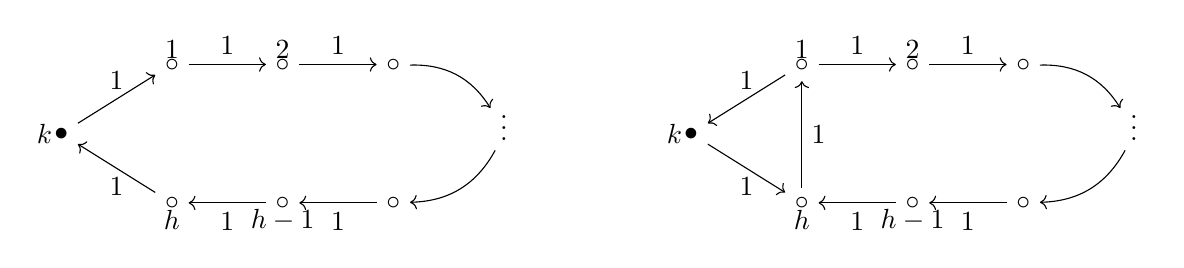
\begin{tikzpicture}[baseline=-0.5ex]
    \matrix[matrix of math nodes,column sep={40pt,between origins},row
    sep={25pt,between origins},nodes={asymmetrical rectangle}] at (0,0)
  {
    & |[name = ul]|\circ& |[name = um]|\circ & |[name = ur]|\circ&\\
    %
    |[name = ml]|\bullet& &&& |[name = mr]|\vdots \\
    %
    & |[name = dl]|\circ& |[name = dm]|\circ & |[name = dr]|\circ&\\
  };
\draw[->]
  (ml) to node[above] {1} (ul)
  ;
  \draw[->]
  (ul) to node[above]{1}(um)
  ;
  \draw[->]
  (um) to node[above]{1}(ur)
  ;
  \draw[->]
  (ur) [bend left] to (mr)
  ;
  \draw[->]
  (mr) [bend left] to (dr)
  ;
  \draw[->]
  (dr) to node[below]{1}(dm)
  ;
  \draw[->]
  (dm) to node[below]{1}(dl)
  ;
  \draw[->]
  (dl) to node[below]{1}(ml)
  ;
    \node at (ml.west){$k$};
    \node at (ul.north){1};
    \node at (um.north){2};
    \node at (dm.south){$h-1$};
    \node at (dl.south){$h$};
    \matrix[matrix of math nodes,column sep={40pt,between origins},row
    sep={25pt,between origins},nodes={asymmetrical rectangle}] at (8,0)
  {
    & |[name = ul]|\circ& |[name = um]|\circ & |[name = ur]|\circ&\\
    %
    |[name = ml]|\bullet& &&& |[name = mr]|\vdots \\
    %
    & |[name = dl]|\circ& |[name = dm]|\circ & |[name = dr]|\circ&\\
  };
\draw[->]
  (ul) to node[above] {1} (ml)
  ;
  \draw[->]
  (ul) to node[above]{1}(um)
  ;
  \draw[->]
  (um) to node[above]{1}(ur)
  ;
  \draw[->]
  (ur) [bend left] to (mr)
  ;
  \draw[->]
  (mr) [bend left] to (dr)
  ;
  \draw[->]
  (dr) to node[below]{1}(dm)
  ;
  \draw[->]
  (dm) to node[below]{1}(dl)
  ;
  \draw[->]
  (ml) to node[below]{1}(dl)
  ;
  \draw[->]
  (dl) to node[right]{1}(ul)
  ;
    \node at (ml.west){$k$};
    \node at (ul.north){1};
    \node at (um.north){2};
    \node at (dm.south){$h-1$};
    \node at (dl.south){$h$};
    \end{tikzpicture}
   
   \item
   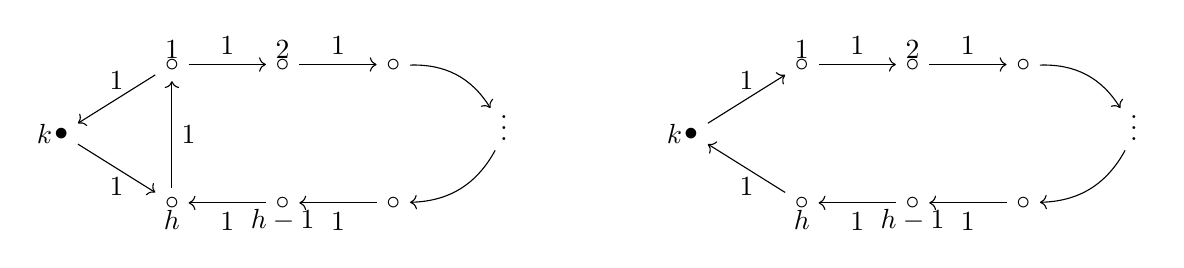
\begin{tikzpicture}[baseline=-0.5ex]
    \matrix[matrix of math nodes,column sep={40pt,between origins},row
    sep={25pt,between origins},nodes={asymmetrical rectangle}] at (8,0)
  {
    & |[name = ul]|\circ& |[name = um]|\circ & |[name = ur]|\circ&\\
    %
    |[name = ml]|\bullet& &&& |[name = mr]|\vdots \\
    %
    & |[name = dl]|\circ& |[name = dm]|\circ & |[name = dr]|\circ&\\
  };
\draw[->]
  (ml) to node[above] {1} (ul)
  ;
  \draw[->]
  (ul) to node[above]{1}(um)
  ;
  \draw[->]
  (um) to node[above]{1}(ur)
  ;
  \draw[->]
  (ur) [bend left] to (mr)
  ;
  \draw[->]
  (mr) [bend left] to (dr)
  ;
  \draw[->]
  (dr) to node[below]{1}(dm)
  ;
  \draw[->]
  (dm) to node[below]{1}(dl)
  ;
  \draw[->]
  (dl) to node[below]{1}(ml)
  ;
    \node at (ml.west){$k$};
    \node at (ul.north){1};
    \node at (um.north){2};
    \node at (dm.south){$h-1$};
    \node at (dl.south){$h$};
    \matrix[matrix of math nodes,column sep={40pt,between origins},row
    sep={25pt,between origins},nodes={asymmetrical rectangle}] at (0,0)
  {
    & |[name = ul]|\circ& |[name = um]|\circ & |[name = ur]|\circ&\\
    %
    |[name = ml]|\bullet& &&& |[name = mr]|\vdots \\
    %
    & |[name = dl]|\circ& |[name = dm]|\circ & |[name = dr]|\circ&\\
  };
\draw[->]
  (ul) to node[above] {1} (ml)
  ;
  \draw[->]
  (ul) to node[above]{1}(um)
  ;
  \draw[->]
  (um) to node[above]{1}(ur)
  ;
  \draw[->]
  (ur) [bend left] to (mr)
  ;
  \draw[->]
  (mr) [bend left] to (dr)
  ;
  \draw[->]
  (dr) to node[below]{1}(dm)
  ;
  \draw[->]
  (dm) to node[below]{1}(dl)
  ;
  \draw[->]
  (ml) to node[below]{1}(dl)
  ;
  \draw[->]
  (dl) to node[right]{1}(ul)
  ;
    \node at (ml.west){$k$};
    \node at (ul.north){1};
    \node at (um.north){2};
    \node at (dm.south){$h-1$};
    \node at (dl.south){$h$};
    \end{tikzpicture}
    
    \item $C$ is an oriented cycle in $\Gamma$ not connected to $k$ and $C'$ is the corresponding cycle in $\Gamma'.$
    
    \item $C$ is an oriented cycle in $\Gamma$ with exactly one vertex in $C$ connected to $k$ by an edge of either weight 1 or 2. Then, $C'$ is the corresponding cycle in $\Gamma'.$  
\end{enumerate}

\end{lem}
\begin{proof}
See \cite[Lemma 2.5]{BM13}.
\end{proof}

\section{The Group of a Diagram in an Artin Group}

\begin{defn}
For $\Gamma$ a diagram of finite type, we define the associated Artin Group as follows. The associated artin group $W_\Gamma$ is generated by $s_i,$ where there is one $s_i$ for each vertex $i$ in $\Gamma.$ These generators are subject to the relations
\begin{itemize}
	\item[(R2')] For all $i \neq j,$ we add the relations
	\\
$	\begin{cases}
	s_is_j=s_js_i, &\text{ if there is no edge between $i$ and $j$}\\
	s_is_js_i = s_js_is_j &\text{ if there is an edge of weight 1 between $i$ and $j.$}\\
	s_is_js_is_j = s_js_is_js_i &\text{ if there is an edge of weight 2 between $i$ and $j$.}\\
	s_is_js_is_js_is_j = s_js_is_js_is_js_i &\text{ if there is an edge of weight 3 between $i$ and $j$.}
\end{cases}$
\item[(R3')(a)] For every chordless cycle of the form

\begin{tikzcd}
i_0 \arrow{r} & i_1 \arrow{r} & \cdots \arrow{r} & i_{d-1} \arrow{r} & i_0
\end{tikzcd}

such that all edges have weight 1, for all $i,$ with $0 \leq a \leq d-1,$ we include the relation 
\begin{align*}
	s_{a}s_{a+1}^{-1}s_{a+2}^{-1}\dots s_{a-2}^{-1}s_{a-1}s_{a-2}s_{a-3}\dots s_{a+1} = s_{a+1}^{-1}\dots s_{a-3}^{-1}s_{a-2}^{-1}s_{a-1}s_{a-2}\dots s_{a+1}s_{a}.
\end{align*}
Where subscripts are taken $\pmod d.$ 

\item[(R3')(a)] For every chordless cycle of the form \begin{tikzpicture}[baseline=-0.5ex]
    \matrix[matrix of math nodes,column sep={25pt,between origins},row
    sep={40pt,between origins},nodes={asymmetrical rectangle}] at (6,0)
  {
    && |[name = u]|\bullet& \\
    %
    &|[name=dl]| \circ & &|[name=dr]| \circ \\
  };
\draw[->]
  (u) to node[right] {1} (dr)
  ;
  \draw[->]
  (dl) to node[left]{2}(u)
  ;
  \draw[->]
  (dr) to node[below]{2}(dl)
  ;
  \node [yshift = .4 cm] at (u){i};
    \node [yshift = -.4 cm,xshift = .4 cm] at (dr){j};
    \node [yshift = -.4 cm,xshift = -.4 cm] at (dl){k};
   \end{tikzpicture}
   we include the three relations
   \begin{enumerate}[(1)]
\item $s_{i}s_{j}^{-1}s_{k}s_{j} = s_{j}^{-1}s_{k}s_{j}s_{i}$
\item $s_{j}s_{k}^{-1}s_{i}s_{k} = s_{k}^{-1}s_{i}s_{k}s_{j}$
\item $s_{k}^{-1}s_{i}^{-1}s_{j}s_{i}s_{k}s_{i}^{-1}s_{j}s_{i}s_{k}^{-1}s_{i}^{-1}s_{j}^{-1}s_{i} = e.$
\end{enumerate}
\end{itemize}
\end{defn}

\begin{rem}
Note that if $\Gamma$ is the graph associated to a dynikin diagram, then $W_\Gamma$ as we have defined it is precisely the corresponding Artin group corresponding to that dynkin diagram. This is the case since in this case we have no cycles in $\Gamma,$ and so we only have relation of the form $(R2'),$ which define the Artin Group.
\end{rem}


\begin{lem}
\label{5.2 analog}
[Proposition 5.2 Analog] The elements $t_i$, for $i$ a vertex of $\Gamma$, satisfy the relations $(R2)$ and $(R3)$.
\end{lem}

After Lemma \ref{lem:one_connected_to_k} we have left to check the relations $(R2)$ when both $i$ and $j$ are connected to $k$ and the relations $(R3)$.  Beginning with the relations $(R2)$, and following cases a-f from Corollary 2.3 in Barot and Marsh:


\begin{enumerate}[a)]
\item
\begin{enumerate}[i)]
\item $$t_it_j = s_ks_is_k^{-1}s_ks_js_k^{-1} = s_ks_is_js_k^{-1} = s_ks_js_is_k^{-1} = t_jt_i$$
\item $$t_it_j = s_is_j = s_js_i = t_jt_i$$
\end{enumerate}
\item
\begin{enumerate}[i)]
\item
\begin{align*}
t_it_jt_i &= s_ks_is_k^{-1}s_js_ks_is_k^{-1}\\
&= s_ks_is_js_ks_j^{-1}s_is_k^{-1}\\
&= s_ks_js_is_ks_is_j^{-1}s_k^{-1}\\
&= s_ks_js_ks_is_ks_j^{-1}s_k^{-1}\\
&= s_js_ks_js_is_j^{-1}s_k^{-1}s_j\\
&= s_js_ks_is_k^{-1}s_j\\
&= t_it_jt_i
\end{align*}

\begin{align*}
t_jt_k^{-1}t_it_k &= s_js_k^{-1}s_ks_is_k^{-1}s_k\\
&= s_js_i\\
&= s_is_j\\
&= t_k^{-1}t_it_kt_j\\
\end{align*}

\item $$t_it_j = s_is_ks_js_k^{-1} = s_is_j^{-1}s_ks_j = s_j^{-1}s_ks_js_i = s_ks_js_k^{-1}s_i = t_jt_i$$
\end{enumerate}
\item
\begin{enumerate}[i)]
\item $$t_it_j = s_ks_is_k^{-1}s_ks_js_k^{-1} = s_ks_is_js_k^{-1} = s_ks_js_is_k^{-1} = t_jt_i$$
\item $$t_it_j = s_is_j = s_js_i = t_jt_i$$
\end{enumerate}
\item
\begin{enumerate}[i)]
\item
\begin{align*}
t_it_jt_it_jt_i^{-1}t_j^{-1}t_i^{-1}t_j^{-1} &= s_ks_is_k^{-1}s_js_ks_is_k^{-1}s_js_ks_i^{-1}s_k^{-1}s_j^{-1}s_ks_i^{-1}s_k^{-1}s_j^{-1}\\
&=s_ks_is_k^{-1}s_js_ks_is_js_ks_j^{-1}s_i^{-1}s_js_k^{-1}s_j^{-1}s_i^{-1}s_k^{-1}s_j^{-1}\\
&=s_ks_is_k^{-1}s_ks_js_ks_is_ks_i^{-1}s_k^{-1}s_j^{-1}s_i^{-1}s_k^{-1}s_j^{-1}\\
&=s_ks_js_is_ks_is_ks_i^{-1}s_k^{-1}s_i^{-1}s_k^{-1}s_j^{-1}s_k^{-1}\\
&= e
\end{align*}

We also have
$$t_jt_k^{-1}t_it_k = s_js_k^{-1}s_ks_is_k^{-1}s_k = s_is_j = t_k^{-1}t_it_kt_j$$ 

\item
\begin{align*}
t_it_j &= s_is_ks_js_k^{-1}\\
&= s_is_j^{-1}s_ks_j\\
&= s_j^{-1}s_ks_js_i\\
&= s_ks_js_k^{-1}s_i\\
&= t_jt_i
\end{align*}
\end{enumerate}
\item
\begin{enumerate}[i)]
\item
\begin{align*}
t_it_jt_it_jt_i^{-1}t_j^{-1}t_i^{-1}t_j^{-1} &= s_ks_is_k^{-1}s_js_ks_is_k^{-1}s_js_ks_i^{-1}s_k^{-1}s_j^{-1}s_ks_i^{-1}s_k^{-1}s_j^{-1}\\
&= s_i^{-1}s_ks_is_js_i^{-1}s_ks_is_js_i^{-1}s_k^{-1}s_is_j^{-1}s_i^{-1}s_k^{-1}s_is_j^{-1}\\
&= s_i^{-1}s_ks_js_ks_js_k^{-1}s_j^{-1}s_k^{-1}s_j^{-1}s_i\\
&= e
\end{align*}
We also have
$$ t_jt_k^{-1}t_it_k = s_js_k^{-1}s_ks_is_k^{-1}s_k = s_js_i = s_is_j = t_it_j$$

\item
\begin{align*}
s_k^{-1}t_it_jt_i^{-1}t_j^{-1}s_k &= s_k^{-1}s_is_ks_js_k^{-1}s_i^{-1}s_ks_j^{-1}\\
&= s_is_ks_i^{-1}s_js_is_k^{-1}s_i^{-1}s_j^{-1}\\
&= e
\end{align*}

\end{enumerate}
\item
\begin{enumerate}[i)]
\item
\begin{align*}
s_k^{-1}t_it_jt_it_j^{-1}t_i^{-1}t_j^{-1} &= s_is_k^{-1}s_js_ks_is_k^{-1}s_j^{-1}s_ks_i^{-1}s_k^{-1}s_j^{-1}s_k\\
&= e
\end{align*}

\begin{align*}
t_it_j^{-1}t_kt_jt_i^{-1}t_j^{-1}s_k^{-1}t_j &= s_ks_is_k^{-1}s_j^{-1}s_ks_js_ks_i^{-1}s_k^{-1}s_j^{-1}s_k^{-1}s_j\\
&= s_ks_is_js_ks_j^{-1}s_k^{-1}s_ks_i^{-1}s_k^{-1}s_j^{-1}s_k^{-1}s_j\\
&= s_ks_is_js_ks_j^{-1}s_i^{-1}s_k^{-1}s_j^{-1}s_k^{-1}s_j\\
&= s_ks_is_js_ks_j^{-1}s_i^{-1}s_js_k^{-1}s_j^{-1}s_k^{-1}\\
&= s_ks_js_ks_j^{-1}s_is_i^{-1}s_js_k^{-1}s_j^{-1}s_k\\
&= e\\
\end{align*}

\item This follows from part (i) by symmetry
\end{enumerate}
\end{enumerate}


\bibliography{References}
\bibliographystyle{alpha}


\end{document}